\section{Registro e Inicio de Sesión}

\subsection{Crear una Cuenta Nueva}
Si es tu primera vez accediendo al portal, debes darte de alta para poder visualizar tus estudios. Sigue estos pasos de manera específica:

\begin{enumerate}
    \item Navega a la página de inicio de sesión de RadiographXpress. En la parte derecha de la pantalla, busca la sección rosa titulada \textbf{"¿No tienes una cuenta?"}.
    \item Localiza la caja (\textit{tarjeta}) que dice \textbf{"Soy Paciente Nuevo"} y haz clic en el botón con letras negras y fondo blanco \textbf{"Crear cuenta de Paciente"}.
    \item Serás redirigido a la pantalla de "Registro". Deberás completar el formulario de dos columnas con los siguientes datos personales y de contacto:
    \begin{itemize}
        \item \textbf{Nombre:} Coloca tus nombres de pila tal y como aparecen en tus documentos de identidad, ya que se utilizarán para validar los estudios.
        \item \textbf{Apellidos:} Ingresa tus apellidos completos.
        \item \textbf{Correo Electrónico:} Inserta una dirección de correo válida a la que tengas acceso. Este será tu usuario principal para iniciar sesión.
        \item \textbf{Dirección:} Coloca tu domicilio actual.
        \item \textbf{Teléfono:} Tu número telefónico a 10 dígitos.
        \item \textbf{Género:} Selecciona tu género biológico/asignado en las opciones desplegables para fines médicos.
        \item \textbf{Contraseña:} Crea una contraseña segura de al menos 8 caracteres. Procura incluir mayúsculas, minúsculas y algún número.
        \item \textbf{Confirmar Contraseña:} Vuelve a escribir tu clave exacta para confirmar que no hay errores tipográficos.
    \end{itemize}
    \item \textbf{Términos y Condiciones:} Antes de continuar, marca la casilla correspondiente indicando que has leído y aceptas los términos, condiciones y la política de privacidad de la clínica.
    \item Haz clic en el botón azul de \textbf{"Crear Cuenta"}. 
    \item \textbf{Verificación:} Si todos tus campos son correctos, el sistema generará tu perfil y te enviará de forma automática un correo electrónico. Ingresa a tu bandeja de entrada (Gmail, Outlook, etc.), busca el mensaje "Activa tu cuenta de RadiographXpress" y haz clic en el enlace de validación para activar tu perfil. Sin este paso, \textbf{no podrás iniciar sesión}. Si no encuentras el correo en tu bandeja de entrada, procura buscar en la sección de \textbf{spam}.
    \begin{figure}[H]
        \centering
        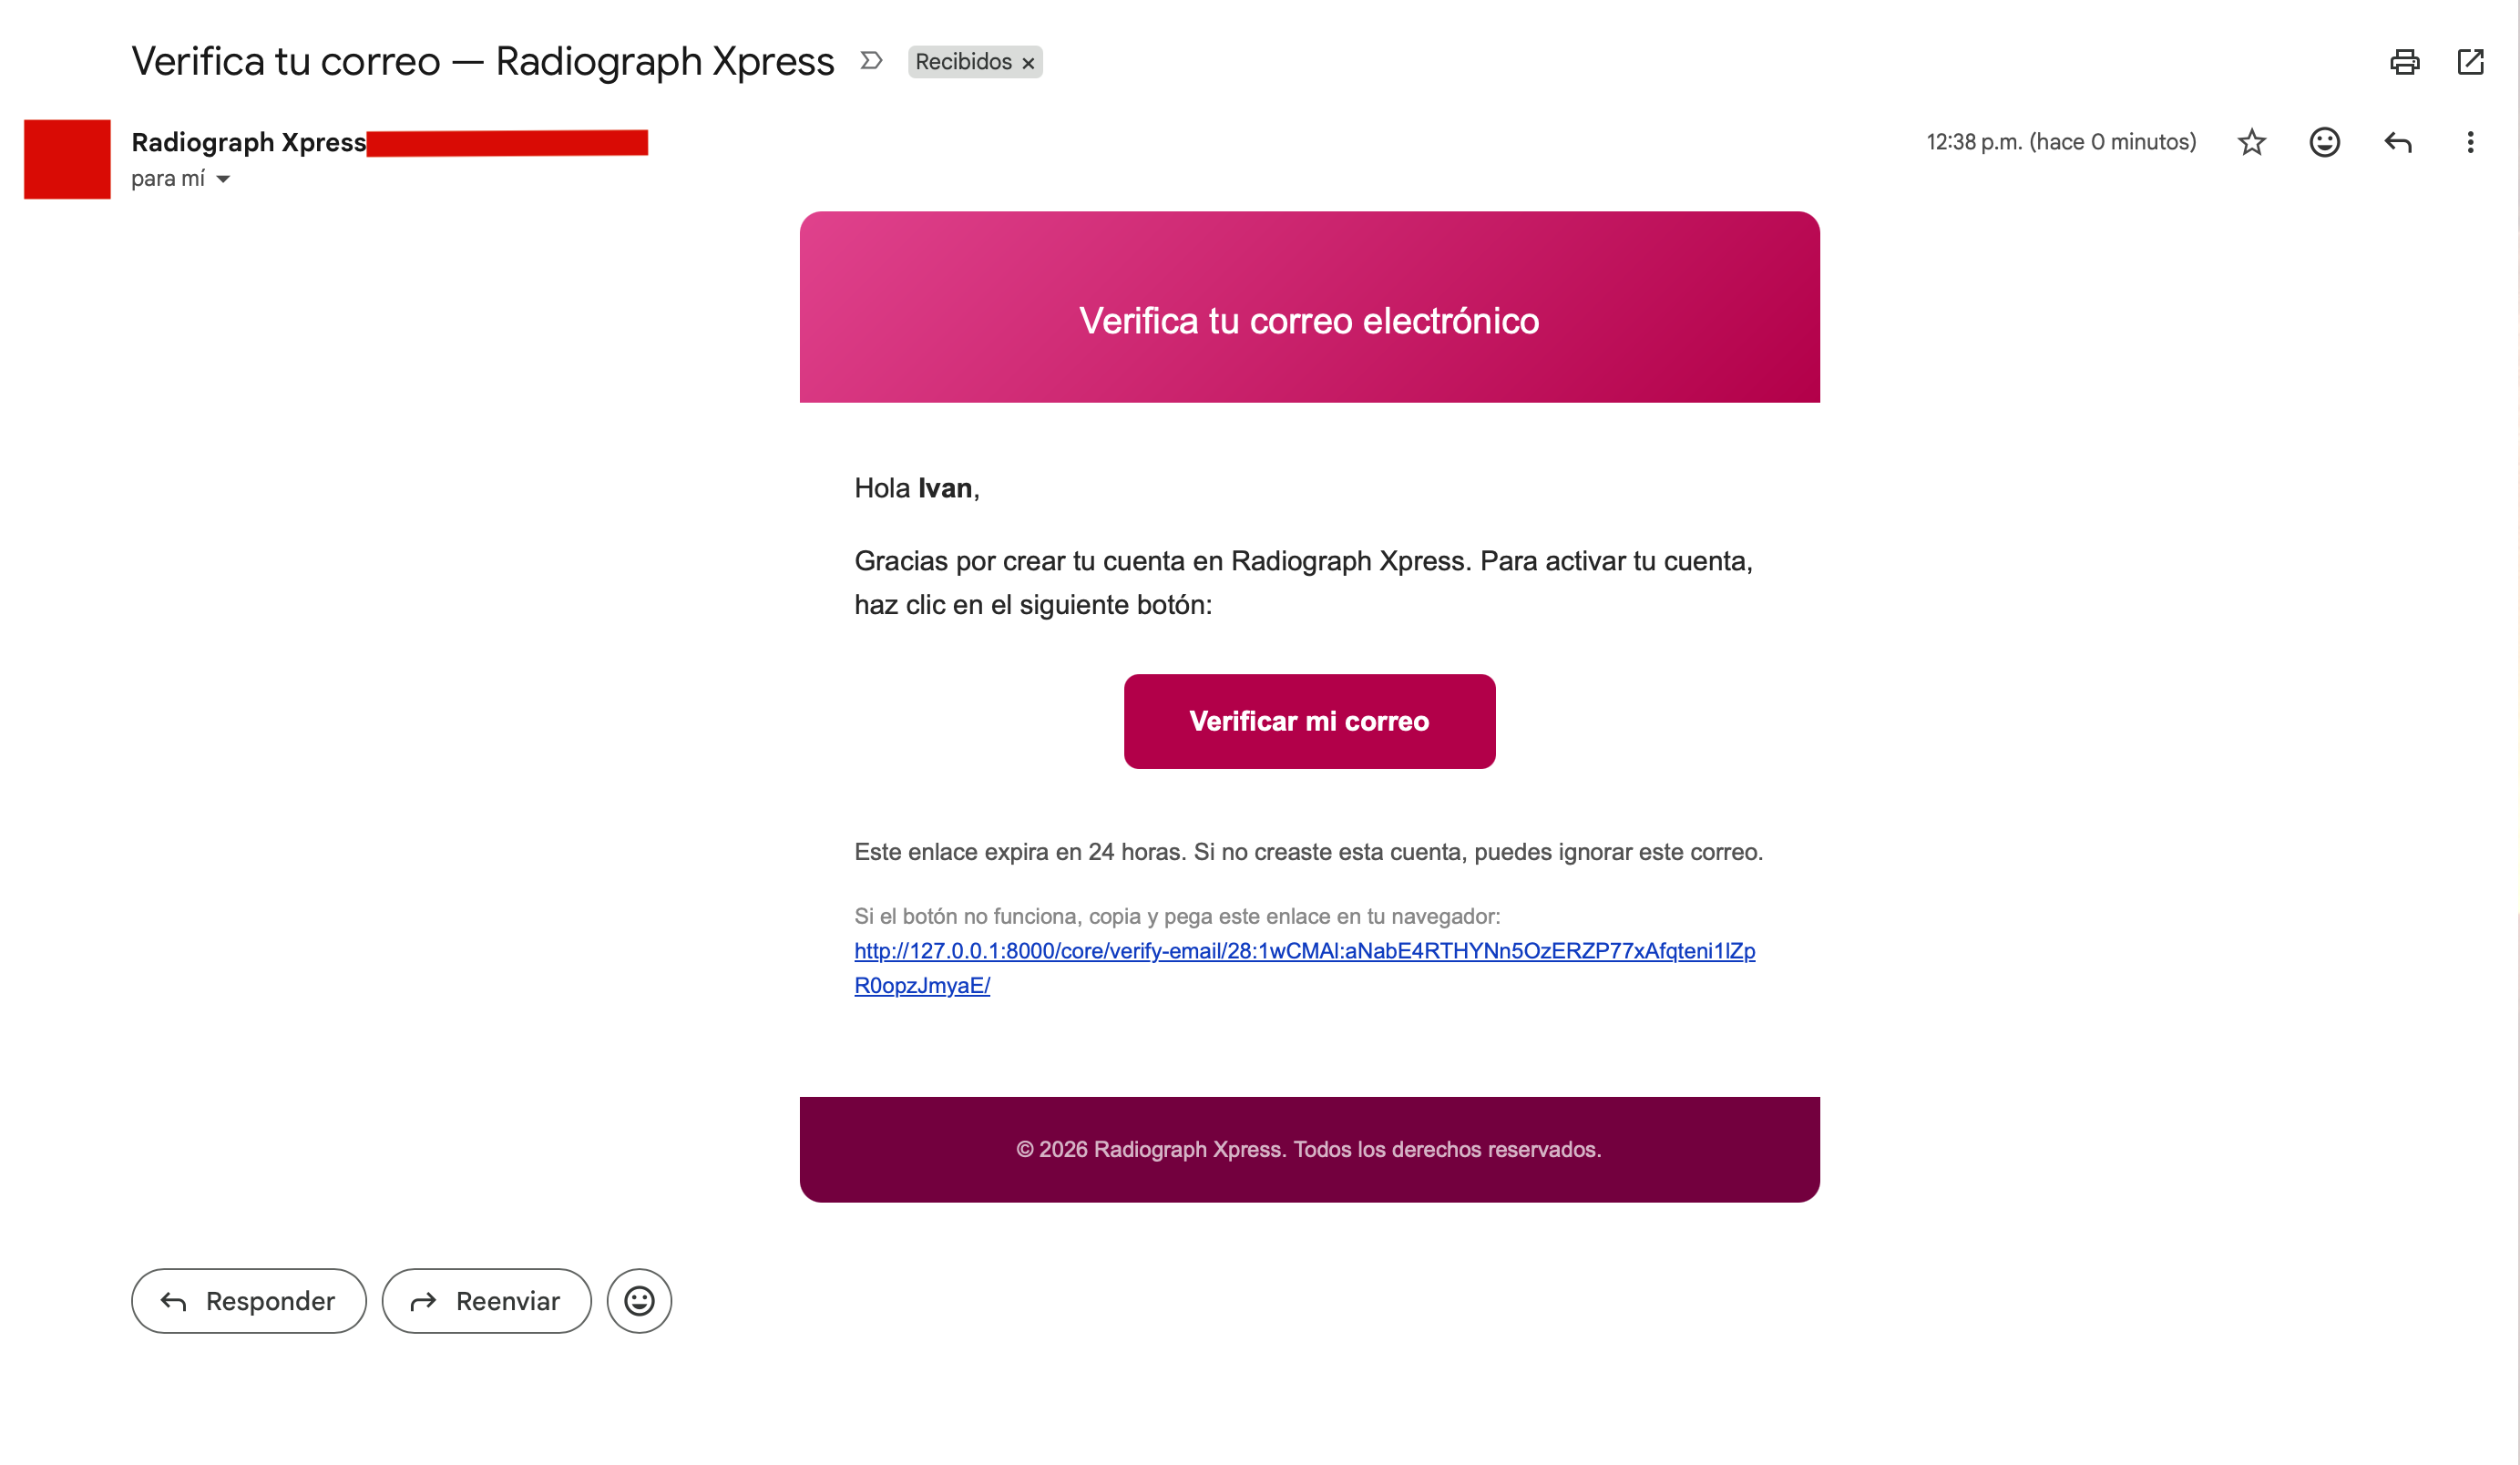
\includegraphics[width=0.5\linewidth]{screenshots/email_verification.png}
        \caption{Ejemplo de email de verificación.}
    \end{figure}
    \item Si la verificación ha sido realizada correctamente, recibiras un nuevo correo electronico, dandote la bienvenida a la plataforma de Radiograph-Xpress.
    \begin{figure}[h]
        \centering
        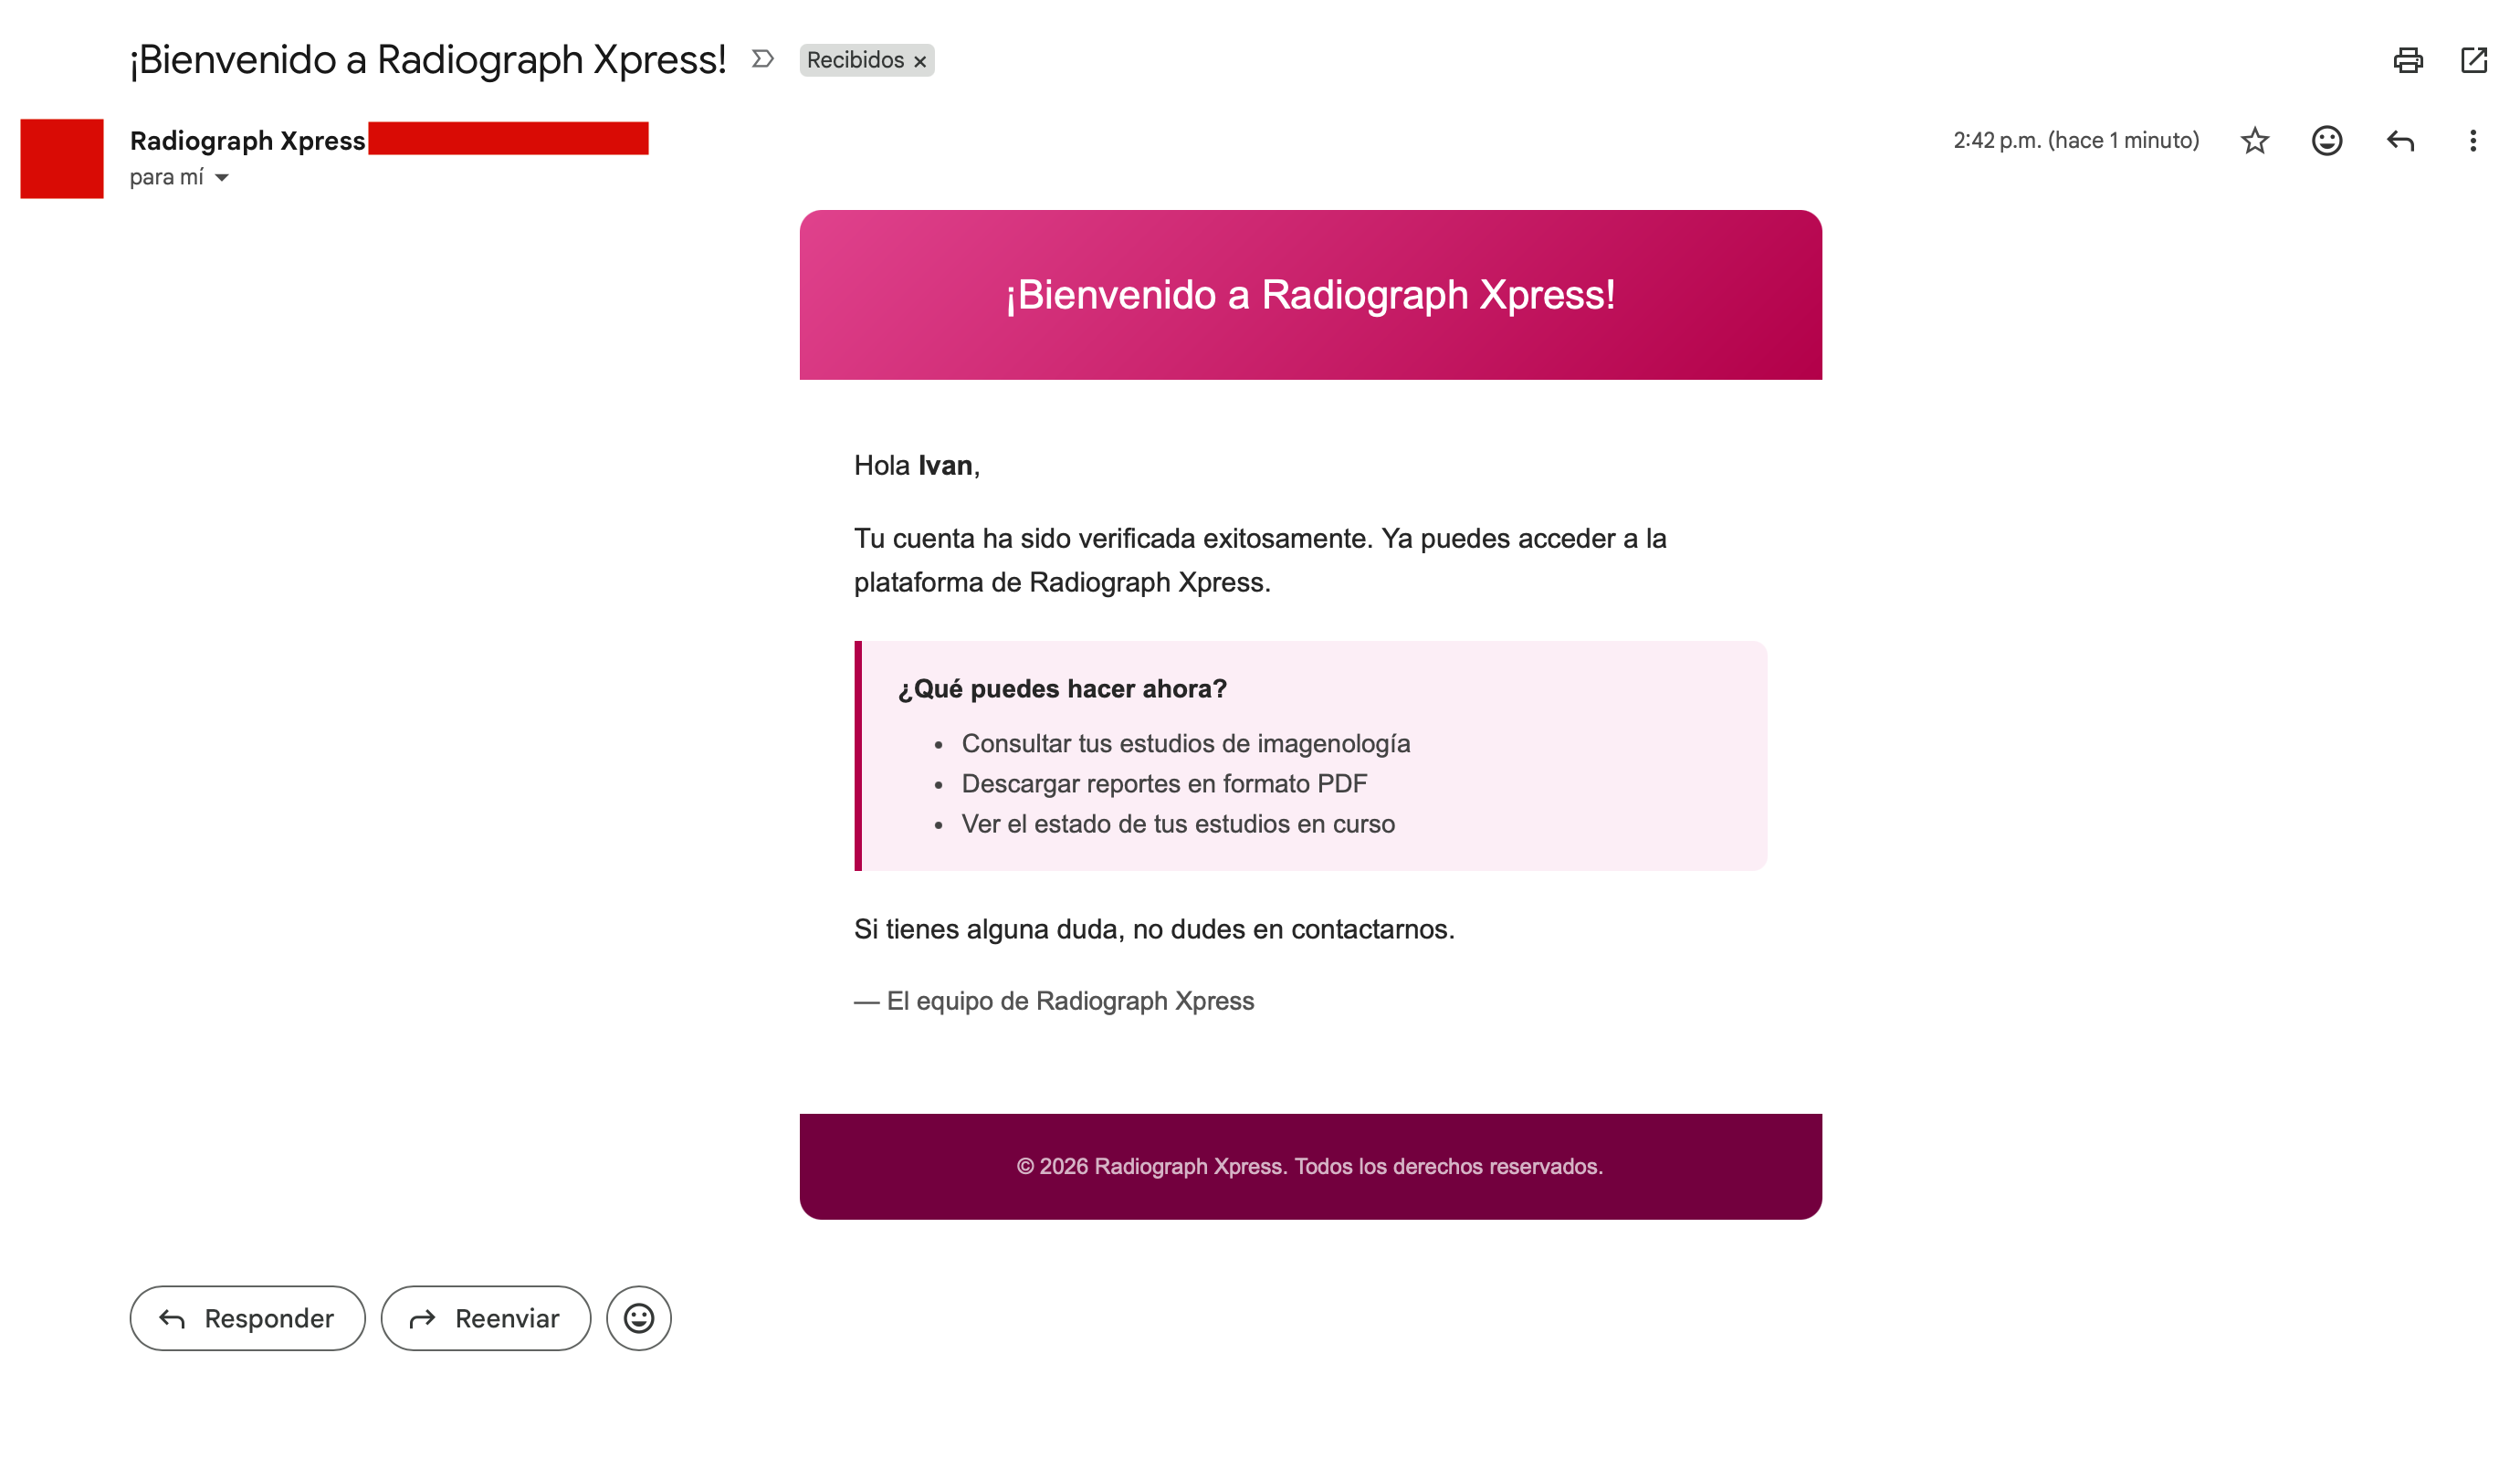
\includegraphics[width=0.5\linewidth]{screenshots/email_welcome.png}
        \caption{Ejemplo de email de bienvenida.}
    \end{figure}
\end{enumerate}

\subsection{Iniciar Sesión Exitoso}
Habiendo validado tu cuenta con el correo electrónico, ahora puedes acceder al sistema de forma regular.

\begin{enumerate}
    \item Regresa a la página de inicio (Login) principal de la clínica en la web.
    \item En la parte izquierda y blanca de la pantalla, encontrarás la caja de formulario debajo de la leyenda \textbf{"Bienvenido de nuevo"}.
    \item En el campo \textbf{Correo Electrónico}, ingresa la cuenta registrada previamente (ej. \textit{ejemplo@correo.com}).
    \item En el campo \textbf{Contraseña}, ingresa tu clave segura generada.
    \begin{itemize}
        \item \textit{Tip de accesibilidad:} Si tienes dudas sobre los caracteres introducidos, presiona el botón con el ícono del "ojo" ubicado en el extremo derecho de la caja de contraseña para revelar su contenido y evitar fallos.
    \end{itemize}
    \item Oprime el botón azul \textbf{"Iniciar Sesión"}.
    \item Si tus credenciales son correctas, el sistema confirmará la autenticación y serás redirigido de manera automática a tu \textbf{Panel Principal ("Dashboard")}, donde estará listado todo tu expediente médico y reportes.
    \begin{figure}[H]
        \centering
        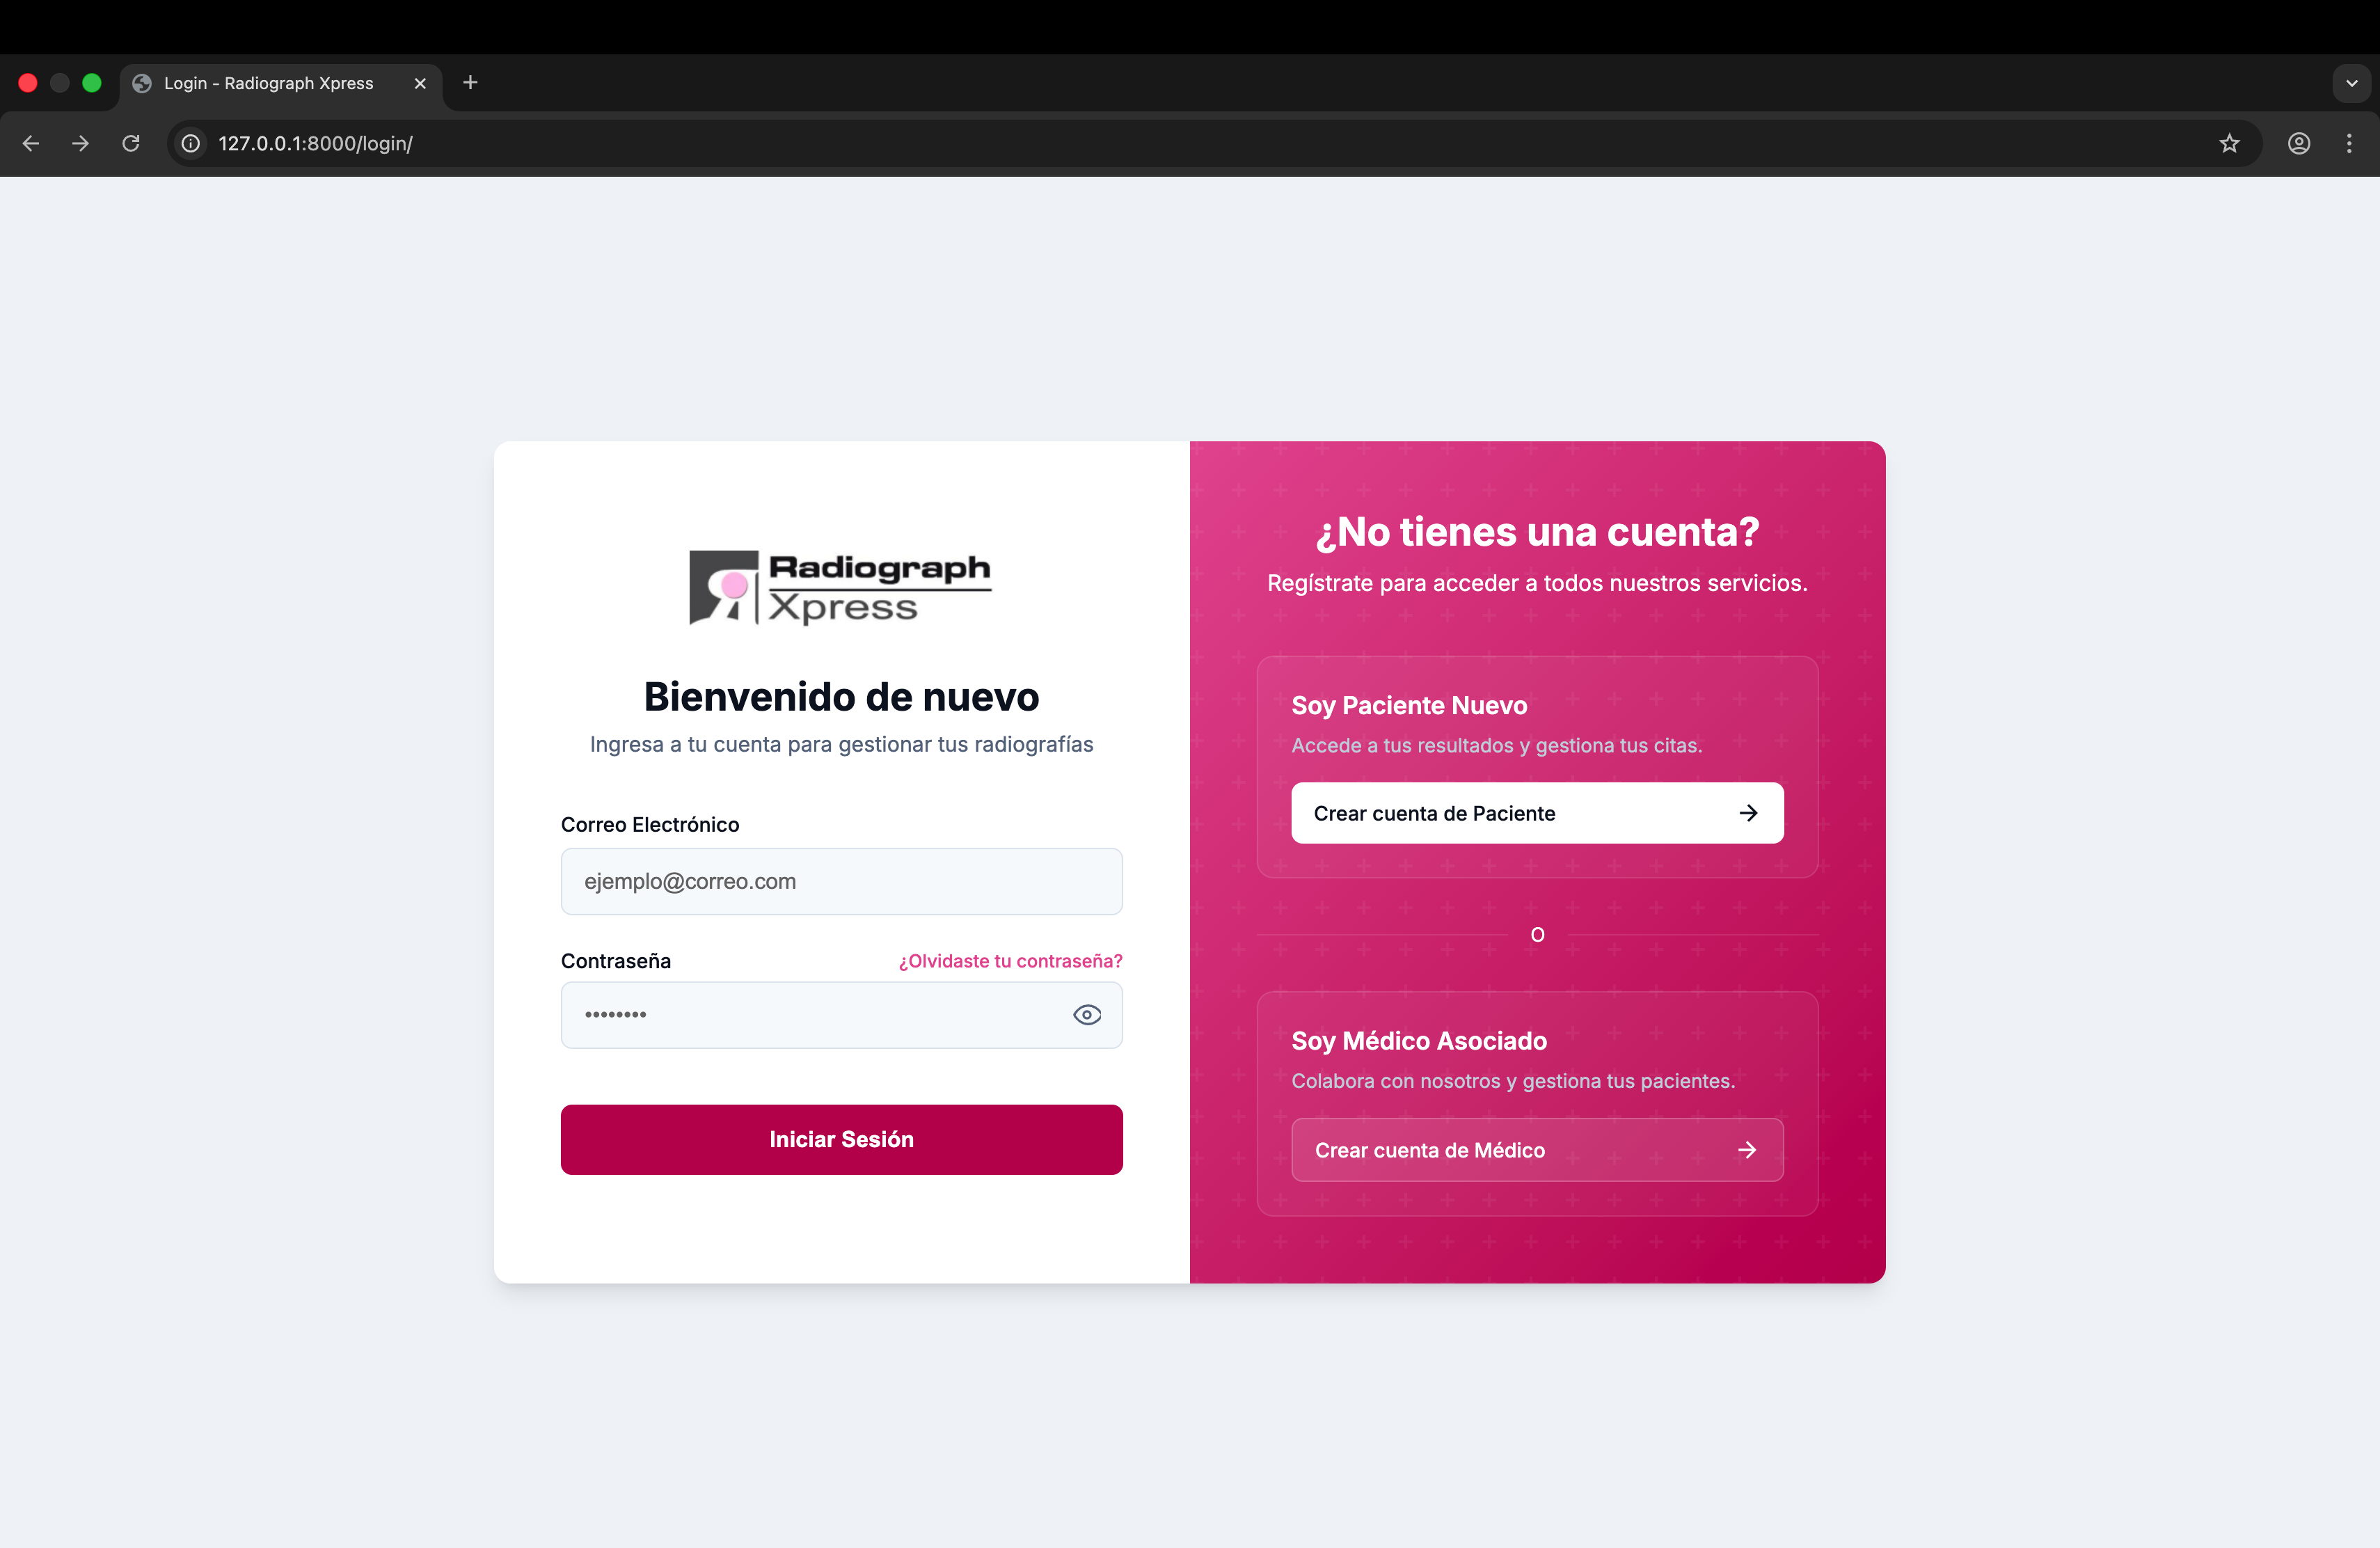
\includegraphics[width=0.7\textwidth]{screenshots/login.png}
        \caption{Pantalla de inicio de sesión.}
    \end{figure}
\end{enumerate}
